

\newpage
\thispagestyle{fancy}
\fancyhf{} % 清空当前的页眉页脚
\setcounter{page}{1}
\fancyfoot[C]{\bfseries\thepage}
\fancyhead[CO]{\bfseries\rightmark}
\fancyhead[RE]{\bfseries\leftmark}
\renewcommand{\headrulewidth}{0.4pt}
\renewcommand{\footrulewidth}{0pt}
\markright{说\ 明\ 书\ 附\ 图}
\section*{图例}
\begin{figure}
  \centering
  % Requires \usepackage{graphicx}
  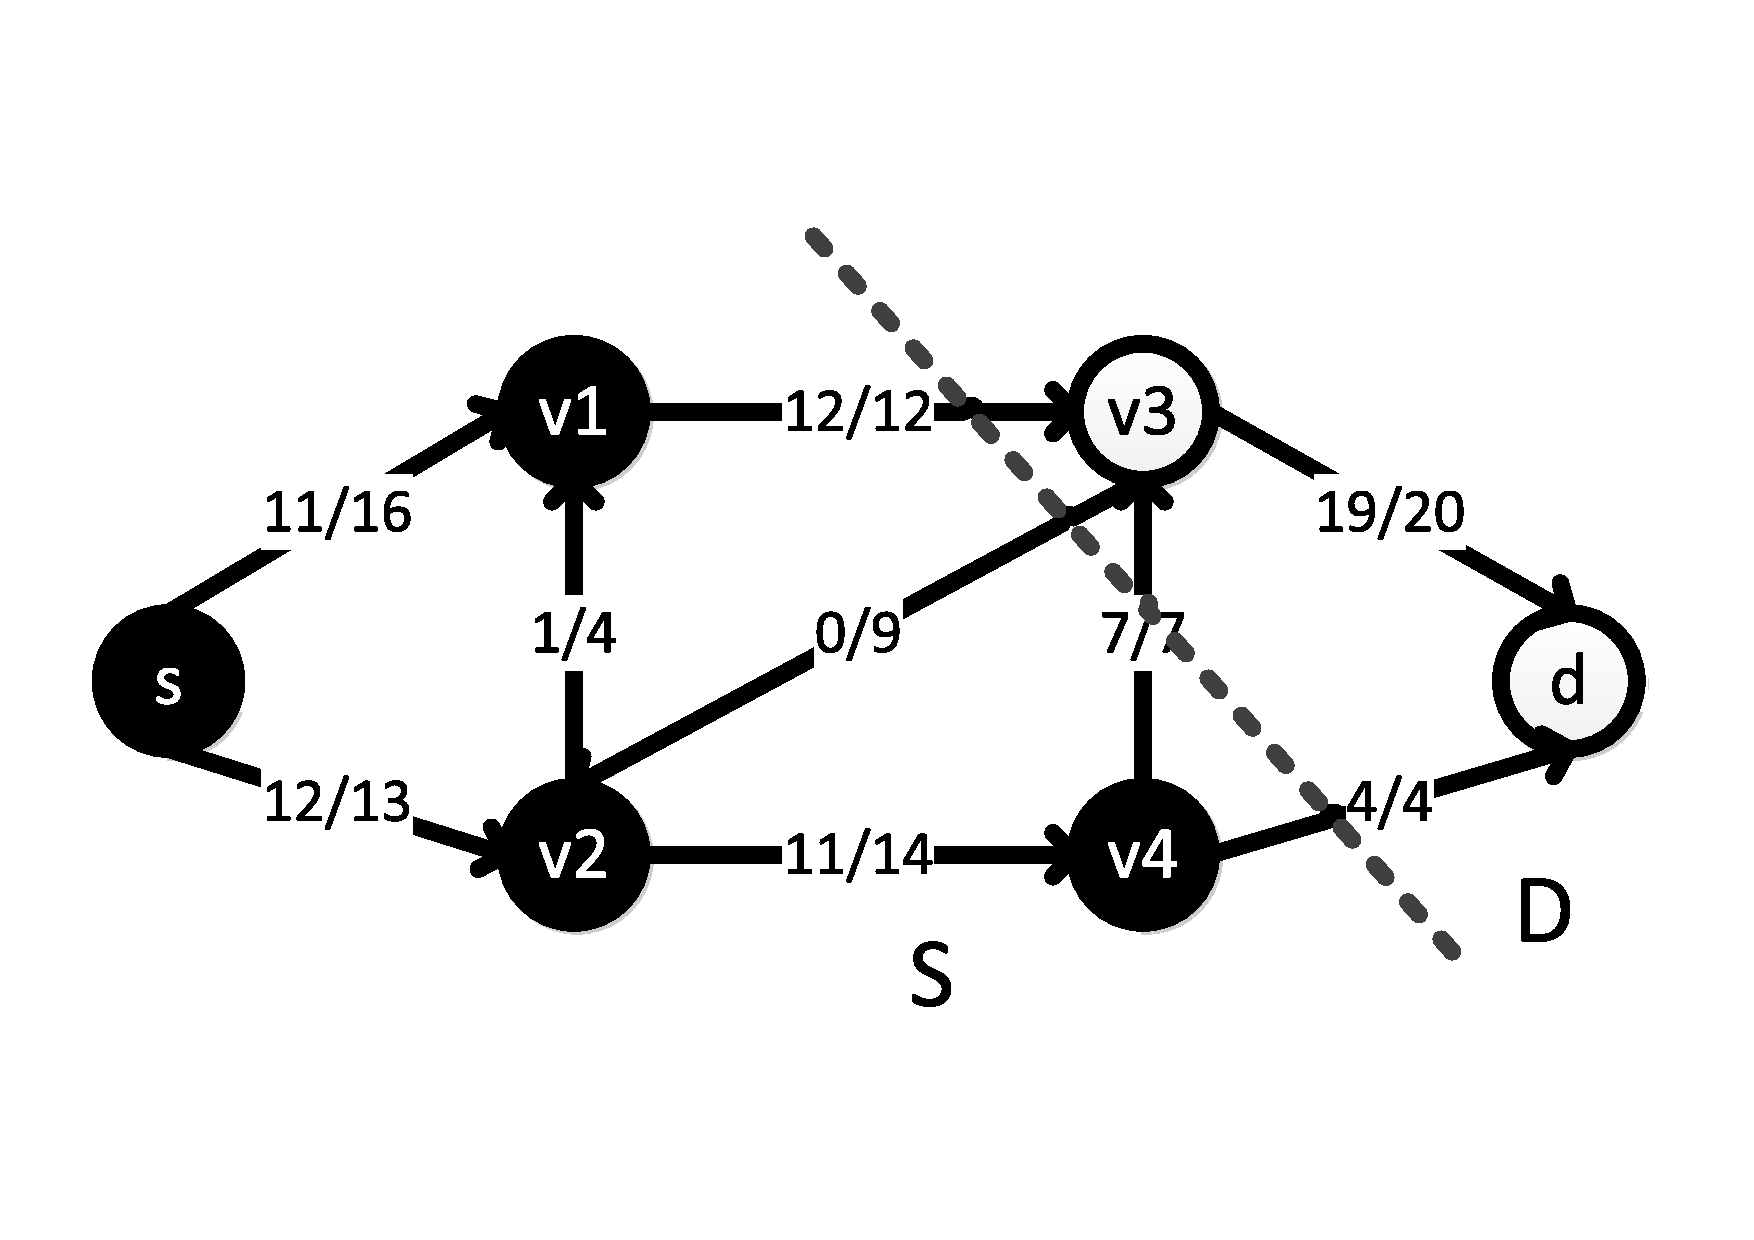
\includegraphics[width=2.5in]{franz//FlowNetwork}\\
  \caption{An example to illustrate max-flow min-cut theorem.}
  \label{fig:FlowNetwork}
\end{figure}
\begin{figure}

  \centering
\subfigure[Physical topology with conduit]{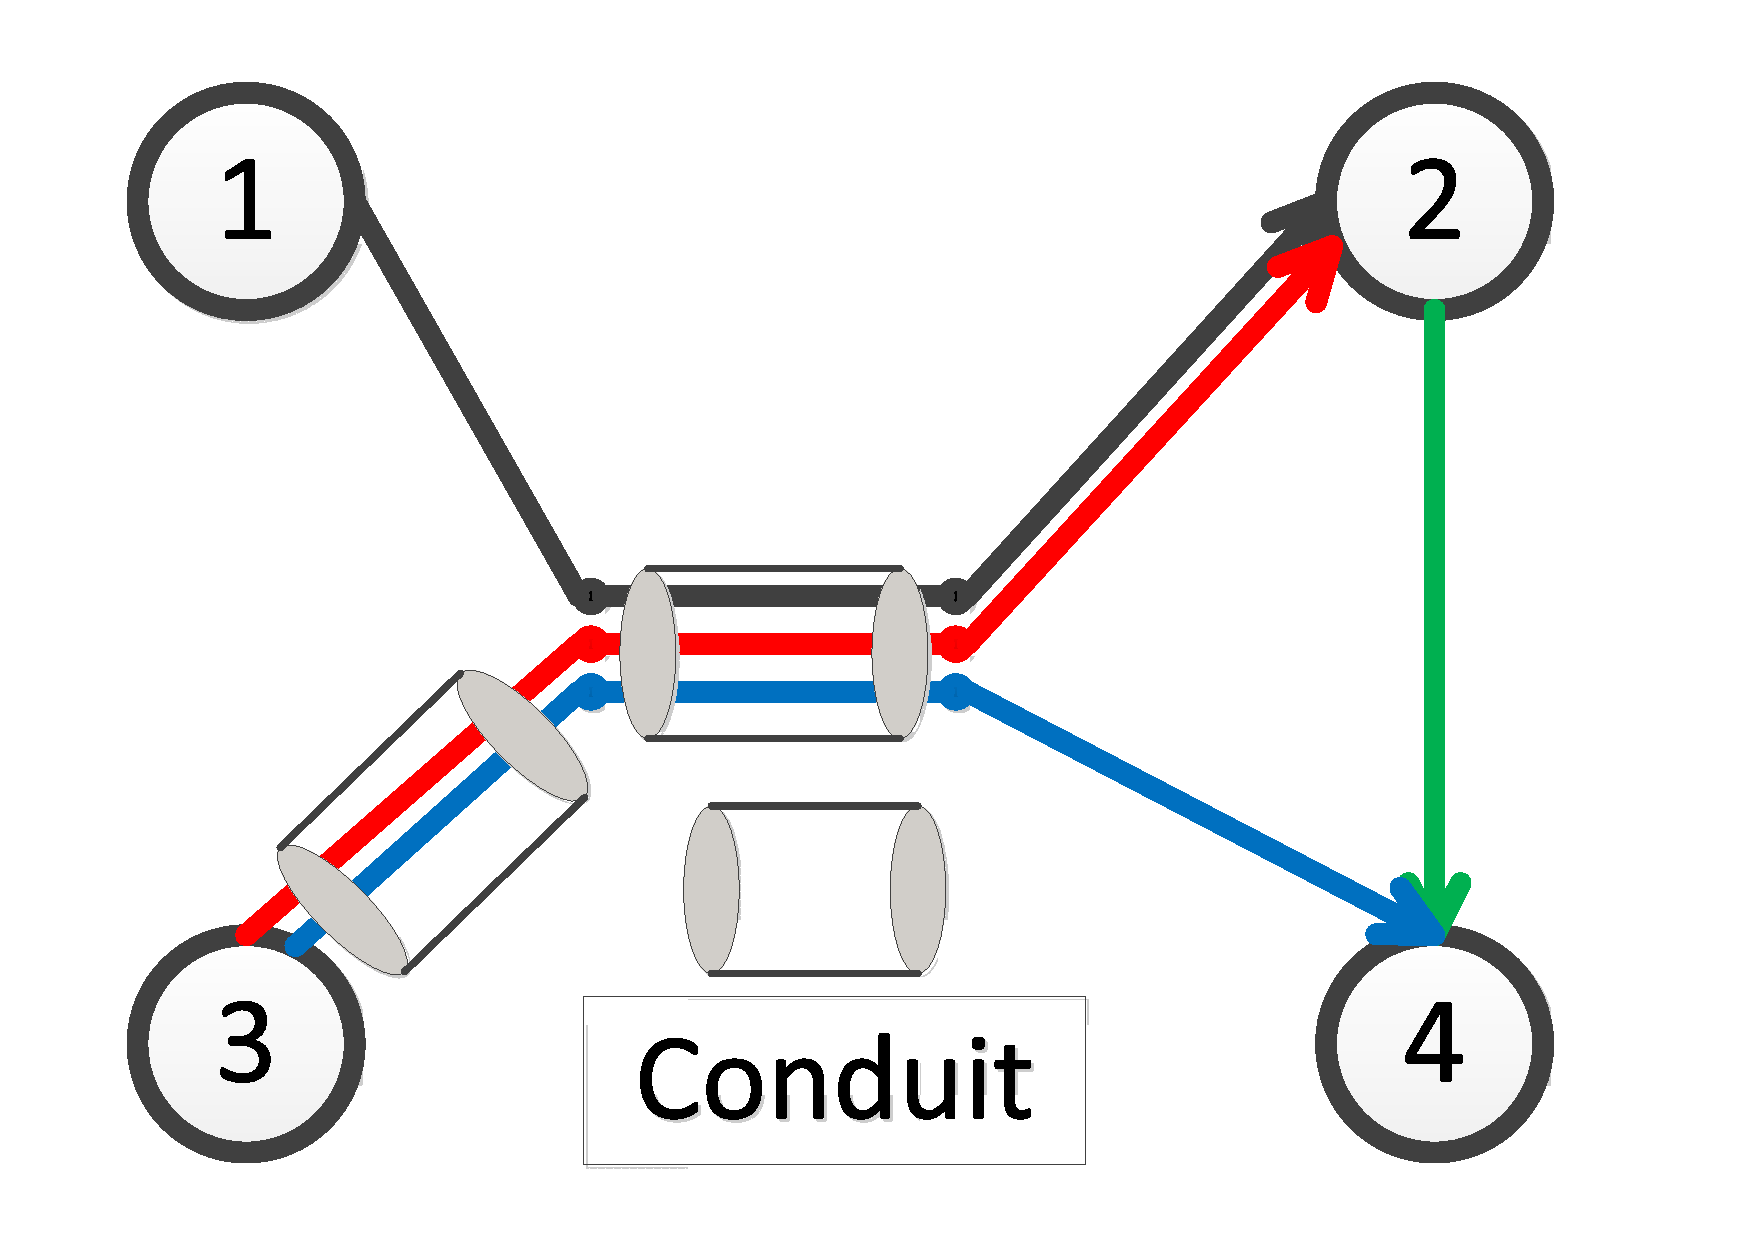
\includegraphics[width=1.65 in]{franz/PhysicalGraph}
}
\subfigure[Network Graph]{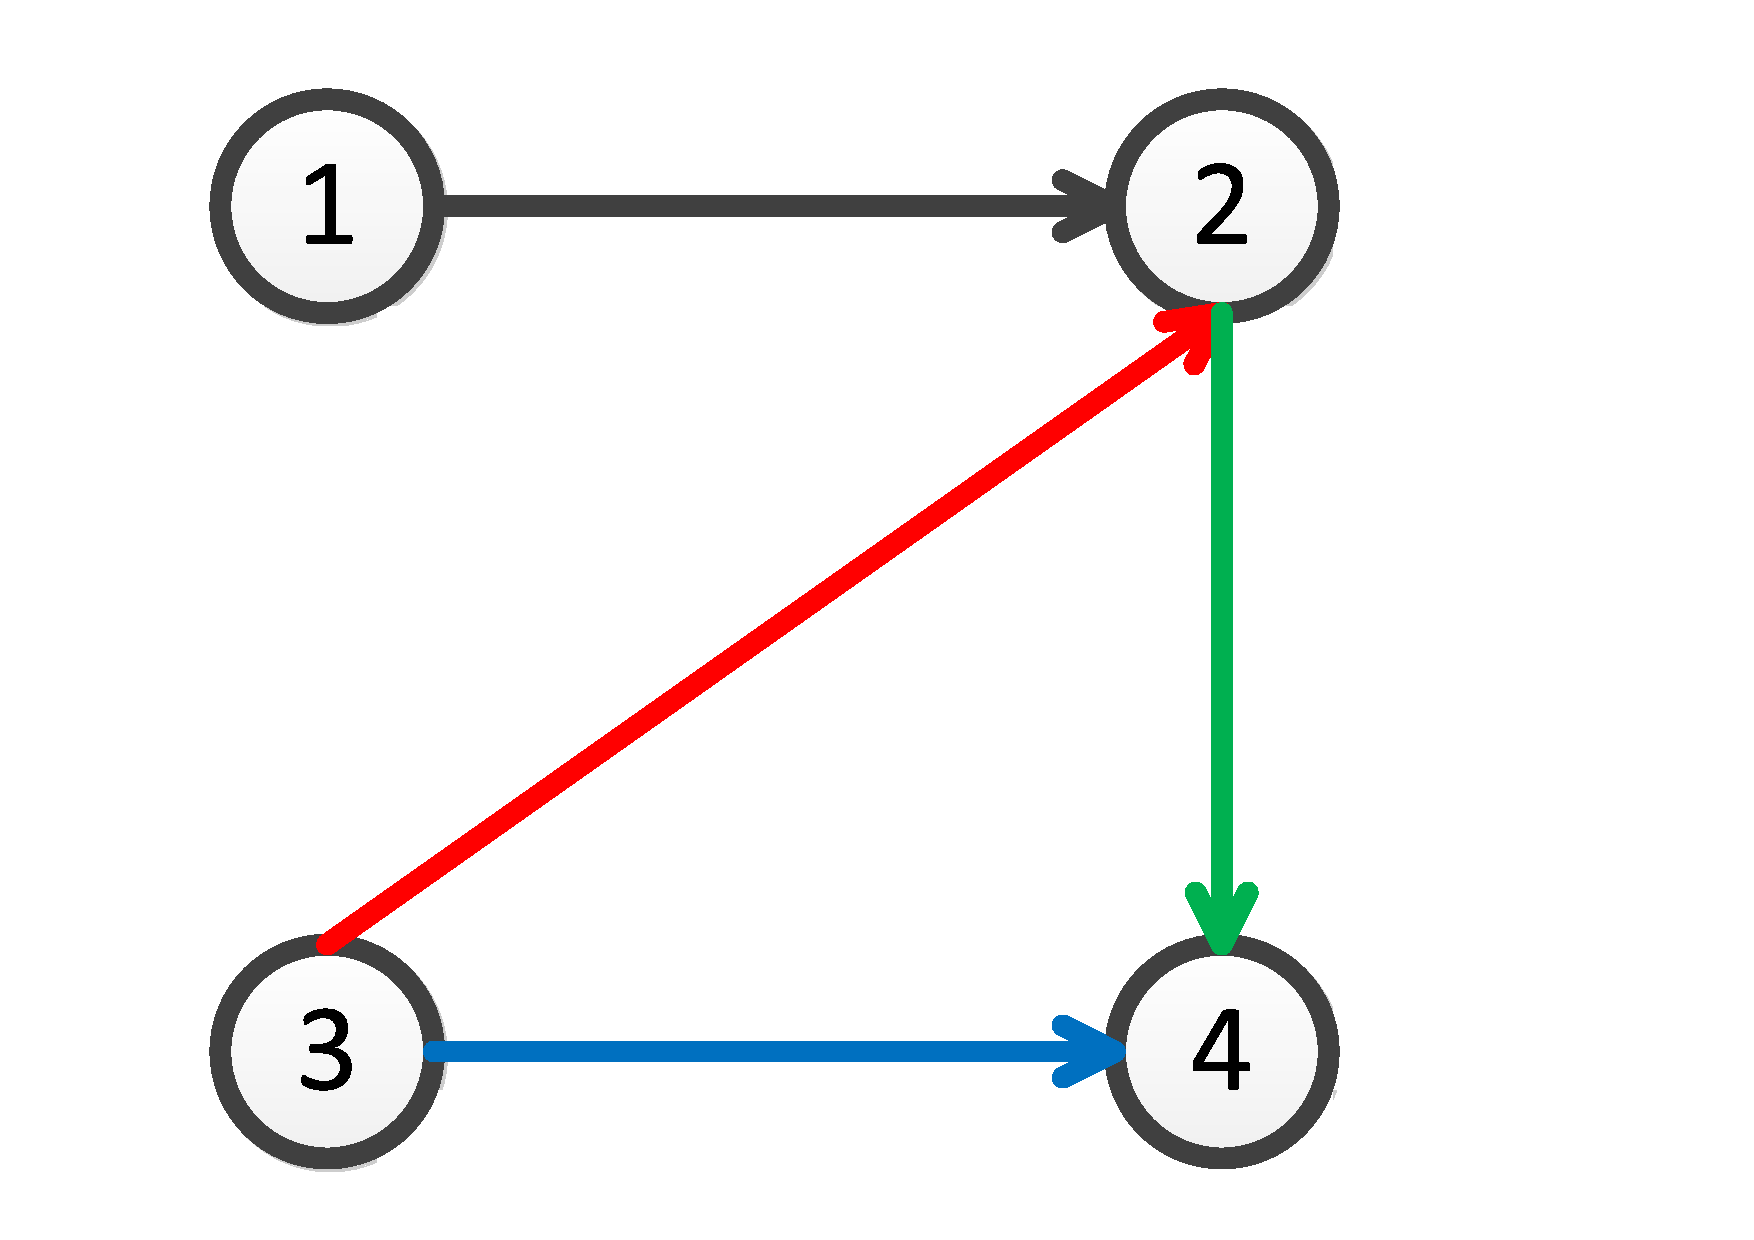
\includegraphics[width=1.40 in]{franz/VirtualGraph}
}
\caption{Example of shared risk link group(SRLG)}\label{fig:SRLGgraph}
\label{fig:Logic shift operation}

\end{figure}
\begin{figure*}[tp]
  \centering
  % Requires \usepackage{graphicx}
  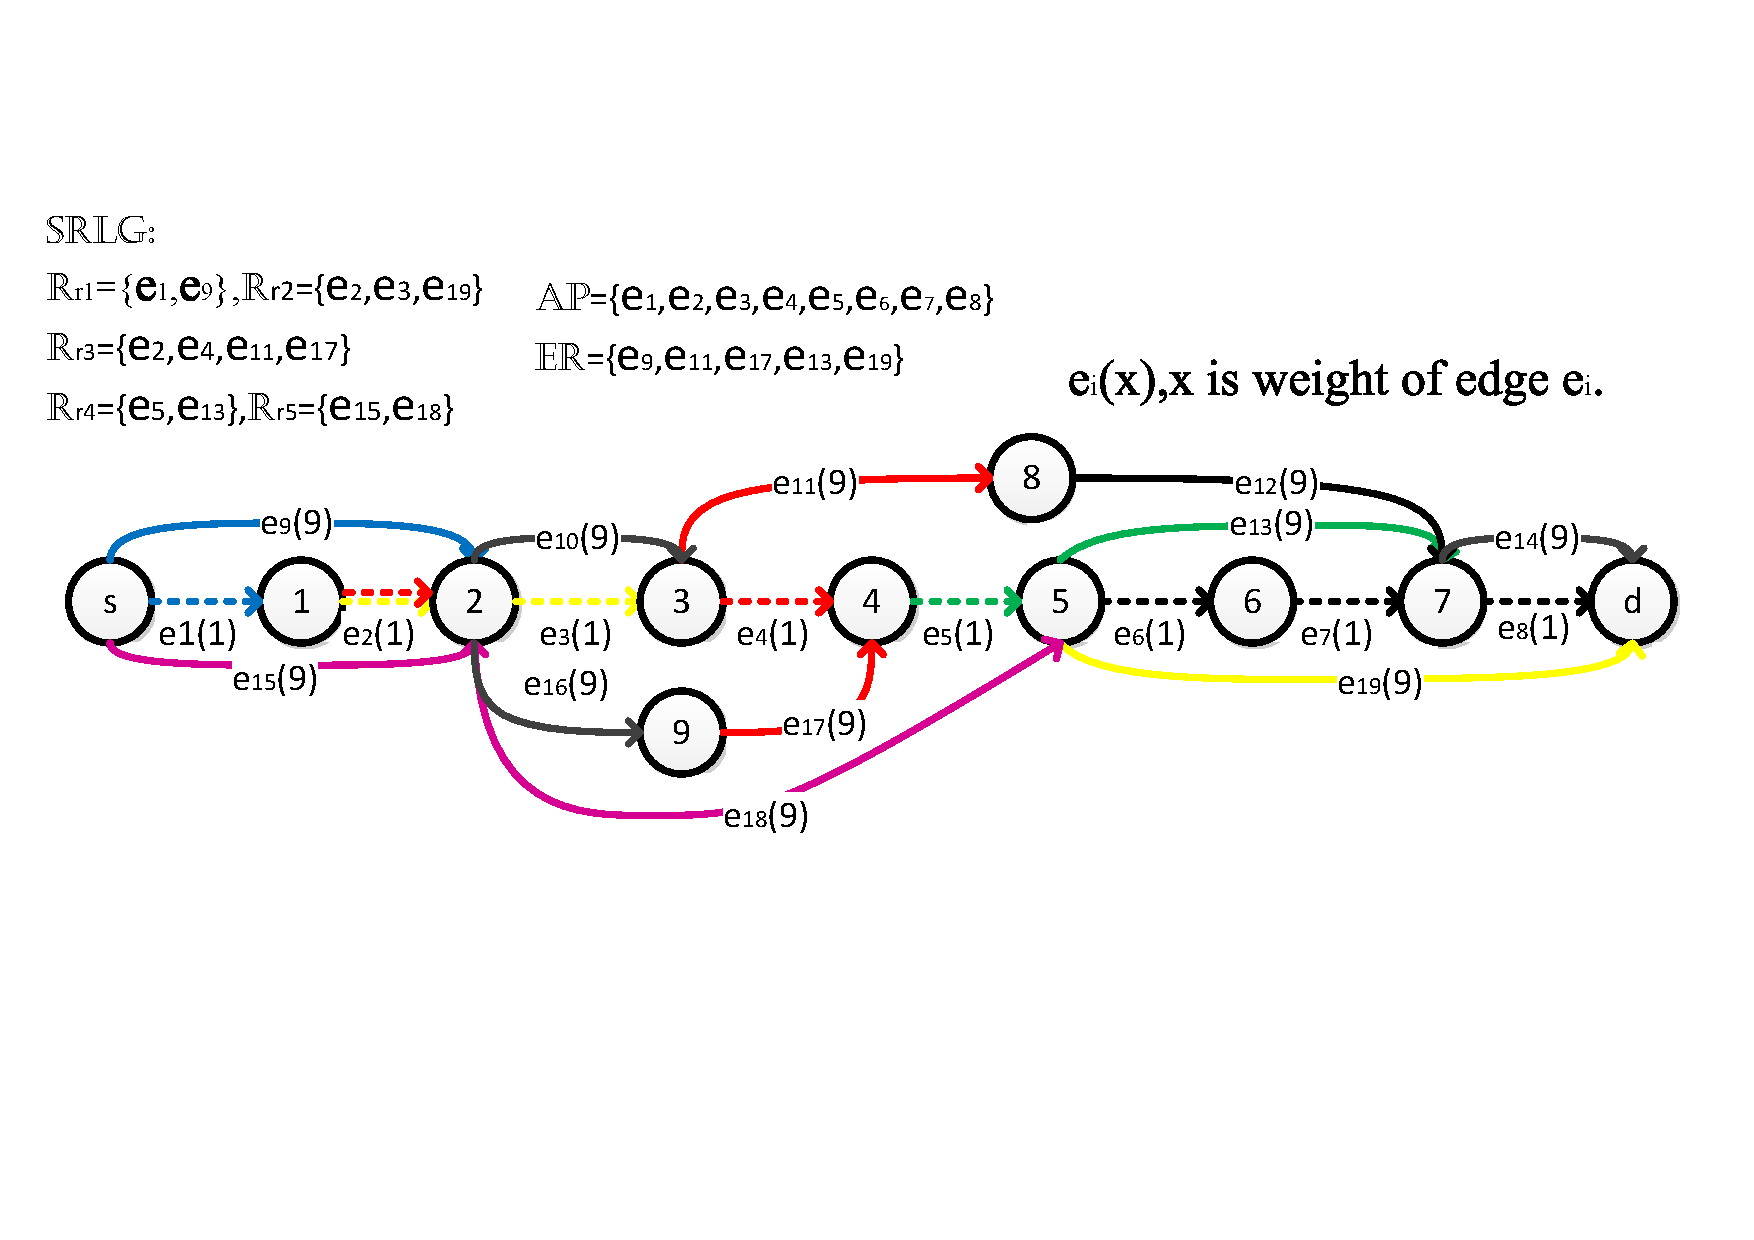
\includegraphics[width=1.35in]{franz/InitialGraph}
  \caption{$\mathbb{AP}=\{e_1,e_2,e_3,e_4,e_5,e_6,e_7,e_8\}$, $\mathbb{\mathbb{ER}}=\{e_9,e_{11},e_{17},e_{13},e_{19}\}$.  SRLGs: $\mathbb{R}_{r_1}=\{e_1,e_9\}$,$\mathbb{R}_{r_2}=\{e_2,e_3,e_{19}\}$,$\mathbb{R}_{r_3}=\{e_2,e_4,e_{11},e_{17}\}$,$\mathbb{R}_{r_4}=\{e_5,e_{13}\}$,$\mathbb{R}_{r_5}=\{e_{15},e_{18}\}$}\label{fig:Initial Graph}
\end{figure*}
\begin{figure*}
  \centering
  % Requires \usepackage{graphicx}
  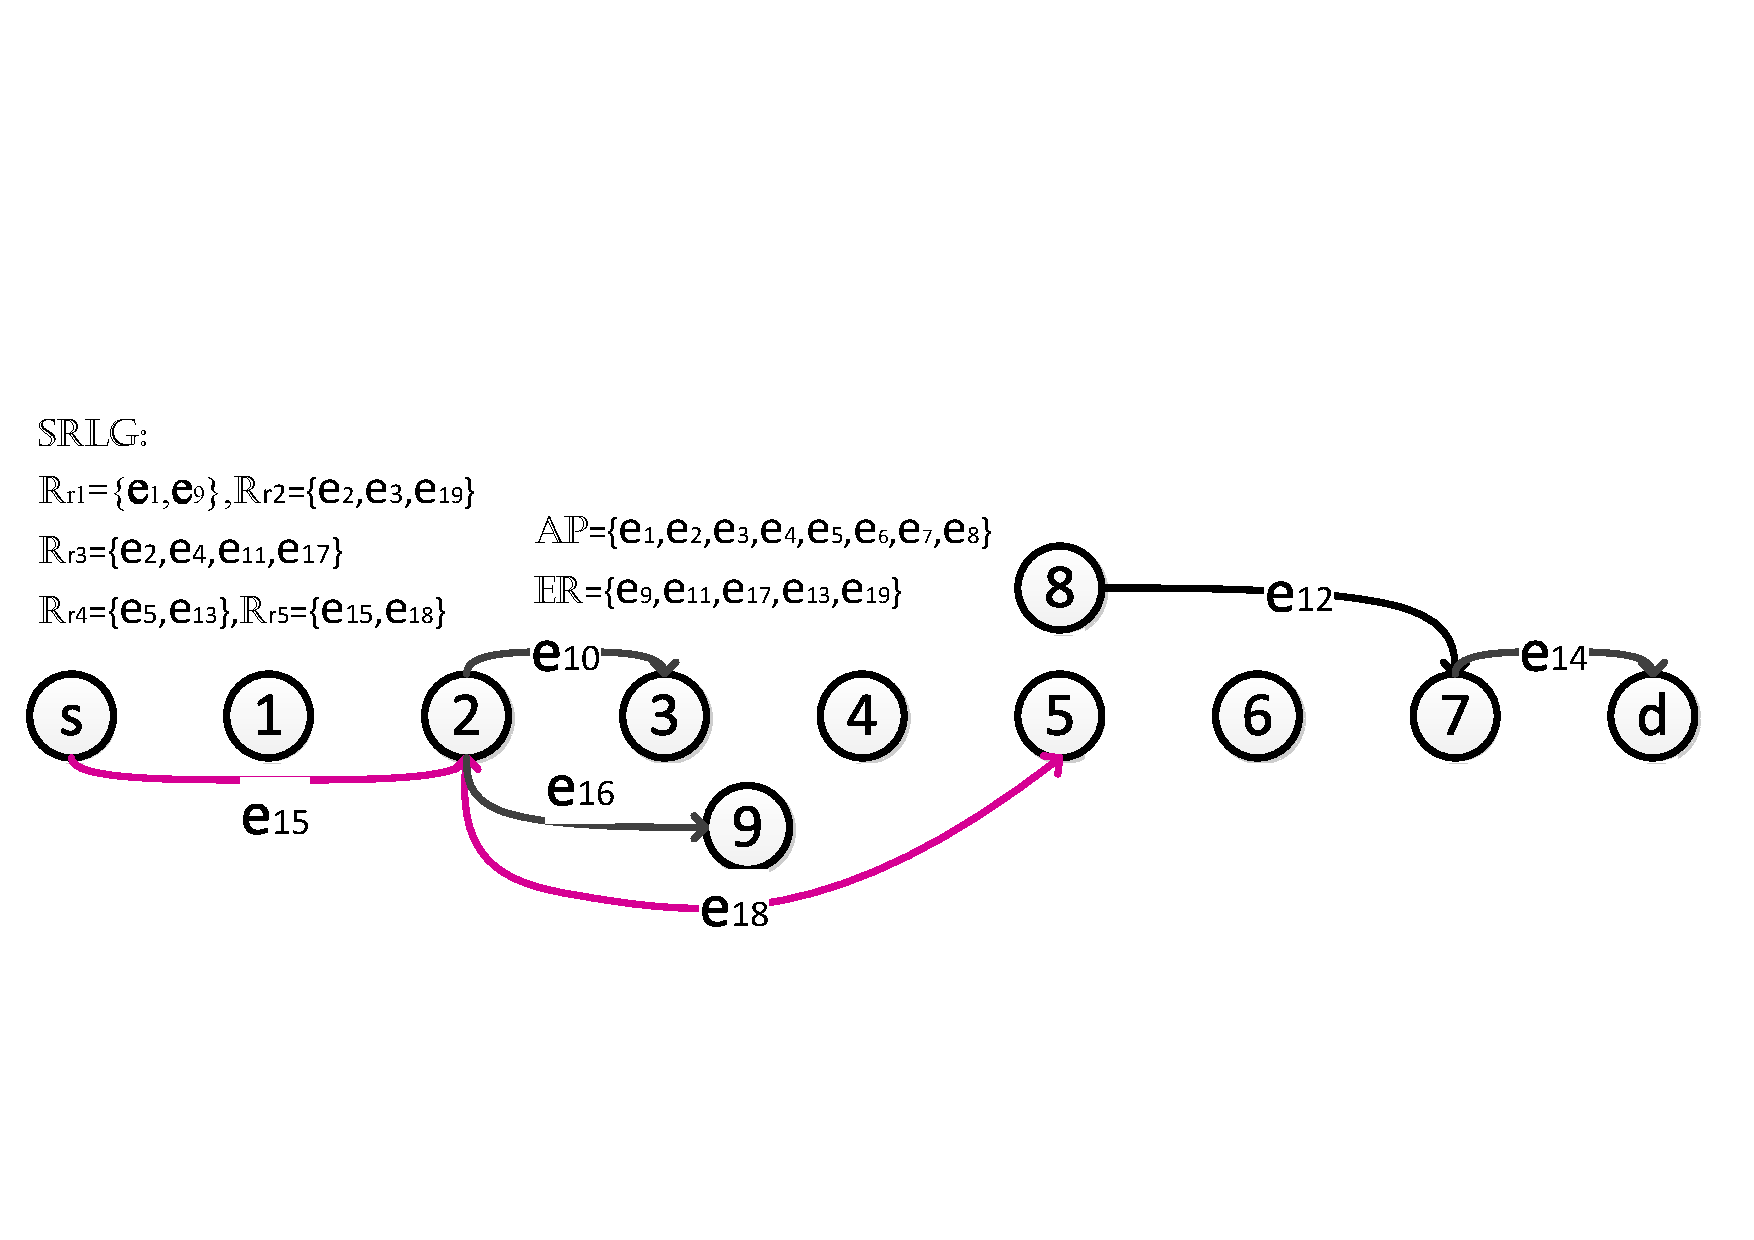
\includegraphics[width=1.35in]{franz/DeletePathGraph}
  \caption{Disconnected graph after deleting the links in $\mathbb{AP}$ and ${\mathbb{ER}}$.}
  \label{fig:DeletePathGraph}
\end{figure*}
\begin{figure}
\tiny{
\begin{equation*}
{\mathcal P}(\emptyset ,\emptyset )\left\{ {\begin{array}{*{20}{l}}
{{\mathcal P}(\{ e2\} ,\emptyset )\left\{ {\begin{array}{*{20}{l}}
{{\mathcal P}(\{ e2,e5\} ,\emptyset )\left\{ {\begin{array}{*{20}{l}}
{{\mathcal P}(\{ e2,e5,e6\} ,\emptyset )}\\
{\boxed{{\mathcal P}(\{ e2,e5\} ,\{ e6\} )}}
\end{array}} \right.}\\
{\boxed{{\mathcal P}(\{ e2\} ,\{ e5\} )}}
\end{array}} \right.}\\
{\boxed{{\mathcal P}(\emptyset ,\{ e2\} )}}
\end{array}} \right.
\end{equation*}
}
\caption{Example to illustrate divide-and-conquer solution}
\label{fig:DividedConquer}
\end{figure}
\begin{figure*}[tp]
  \centering
  % Requires \usepackage{graphicx}
  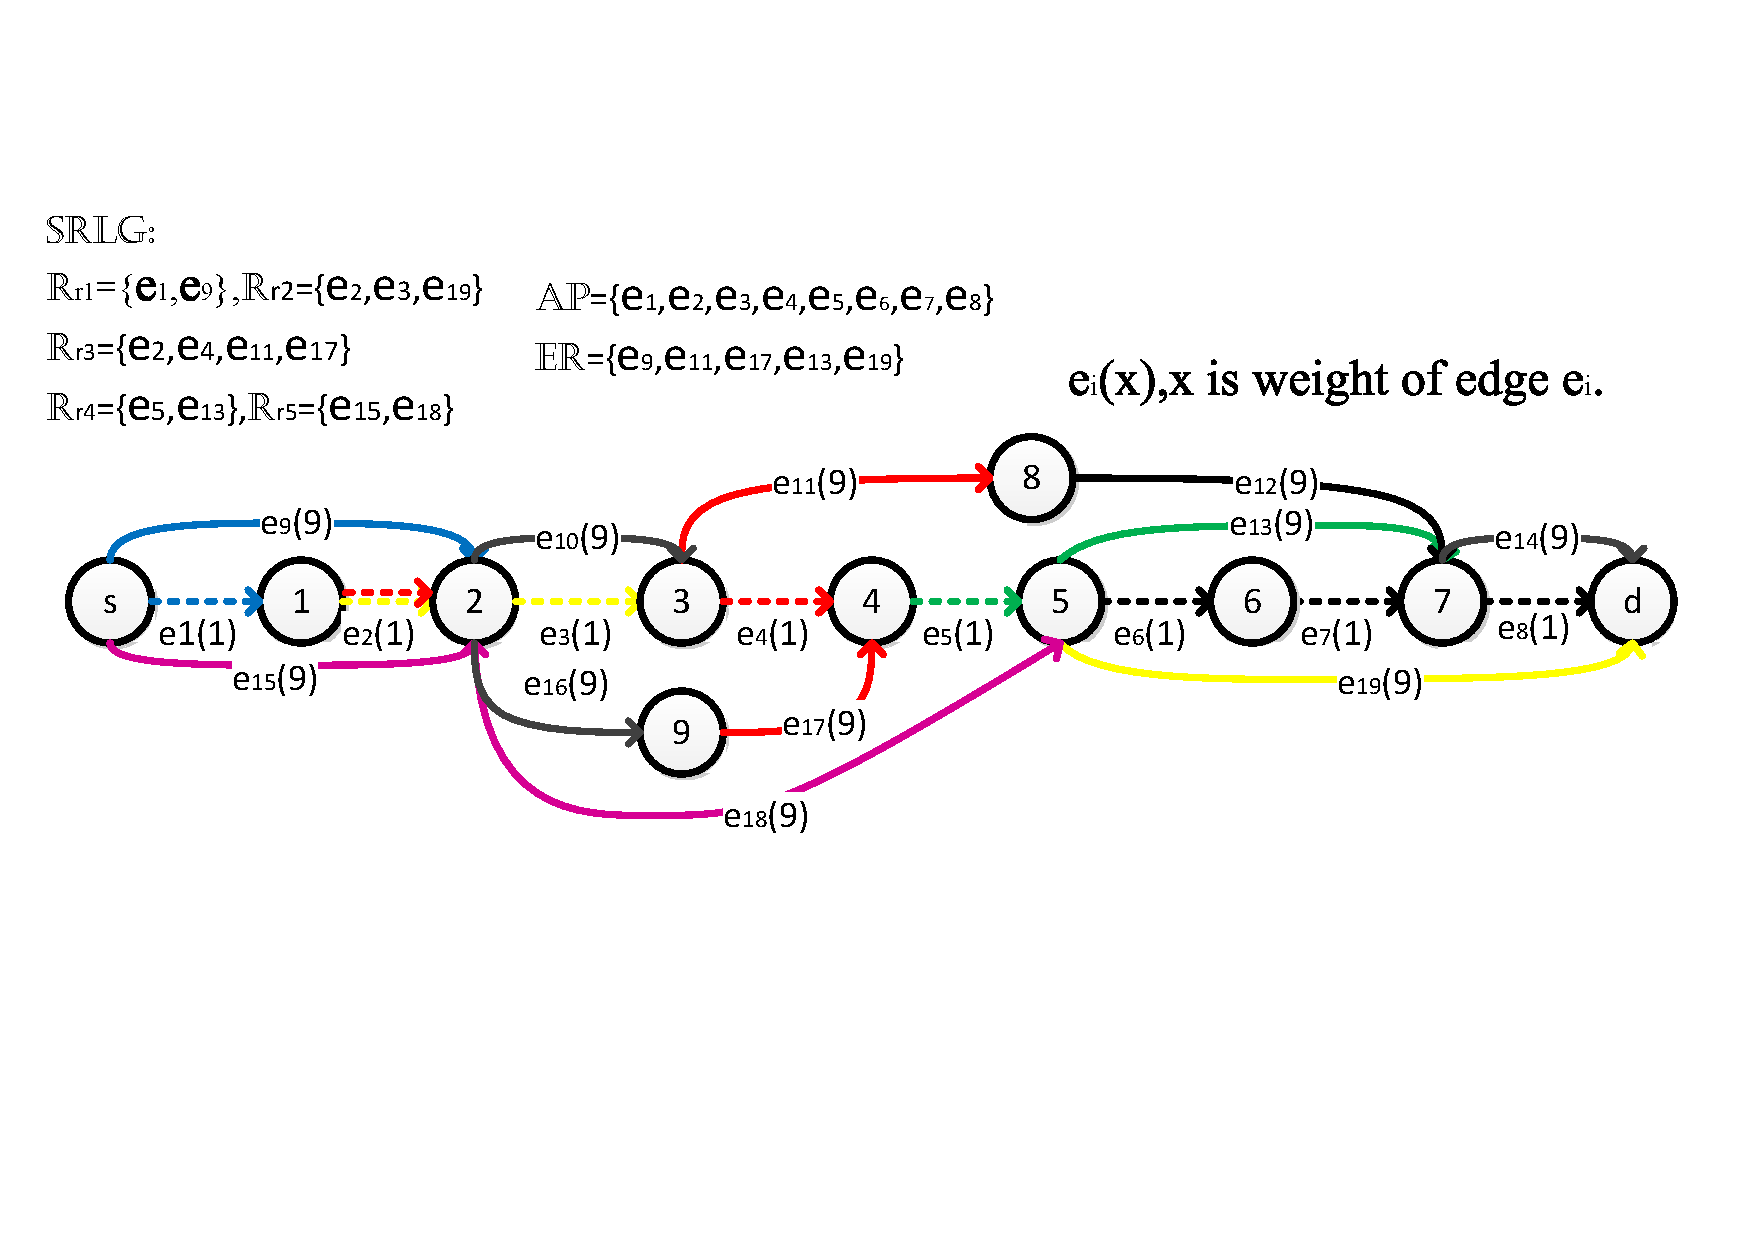
\includegraphics[width=1.35in]{franz/FlowStarGraph}
  \caption{New Graph $G^*$}\label{fig:FlowStarGraph}
\end{figure*}

\begin{figure*}[tp]
  \centering
  % Requires \usepackage{graphicx}
  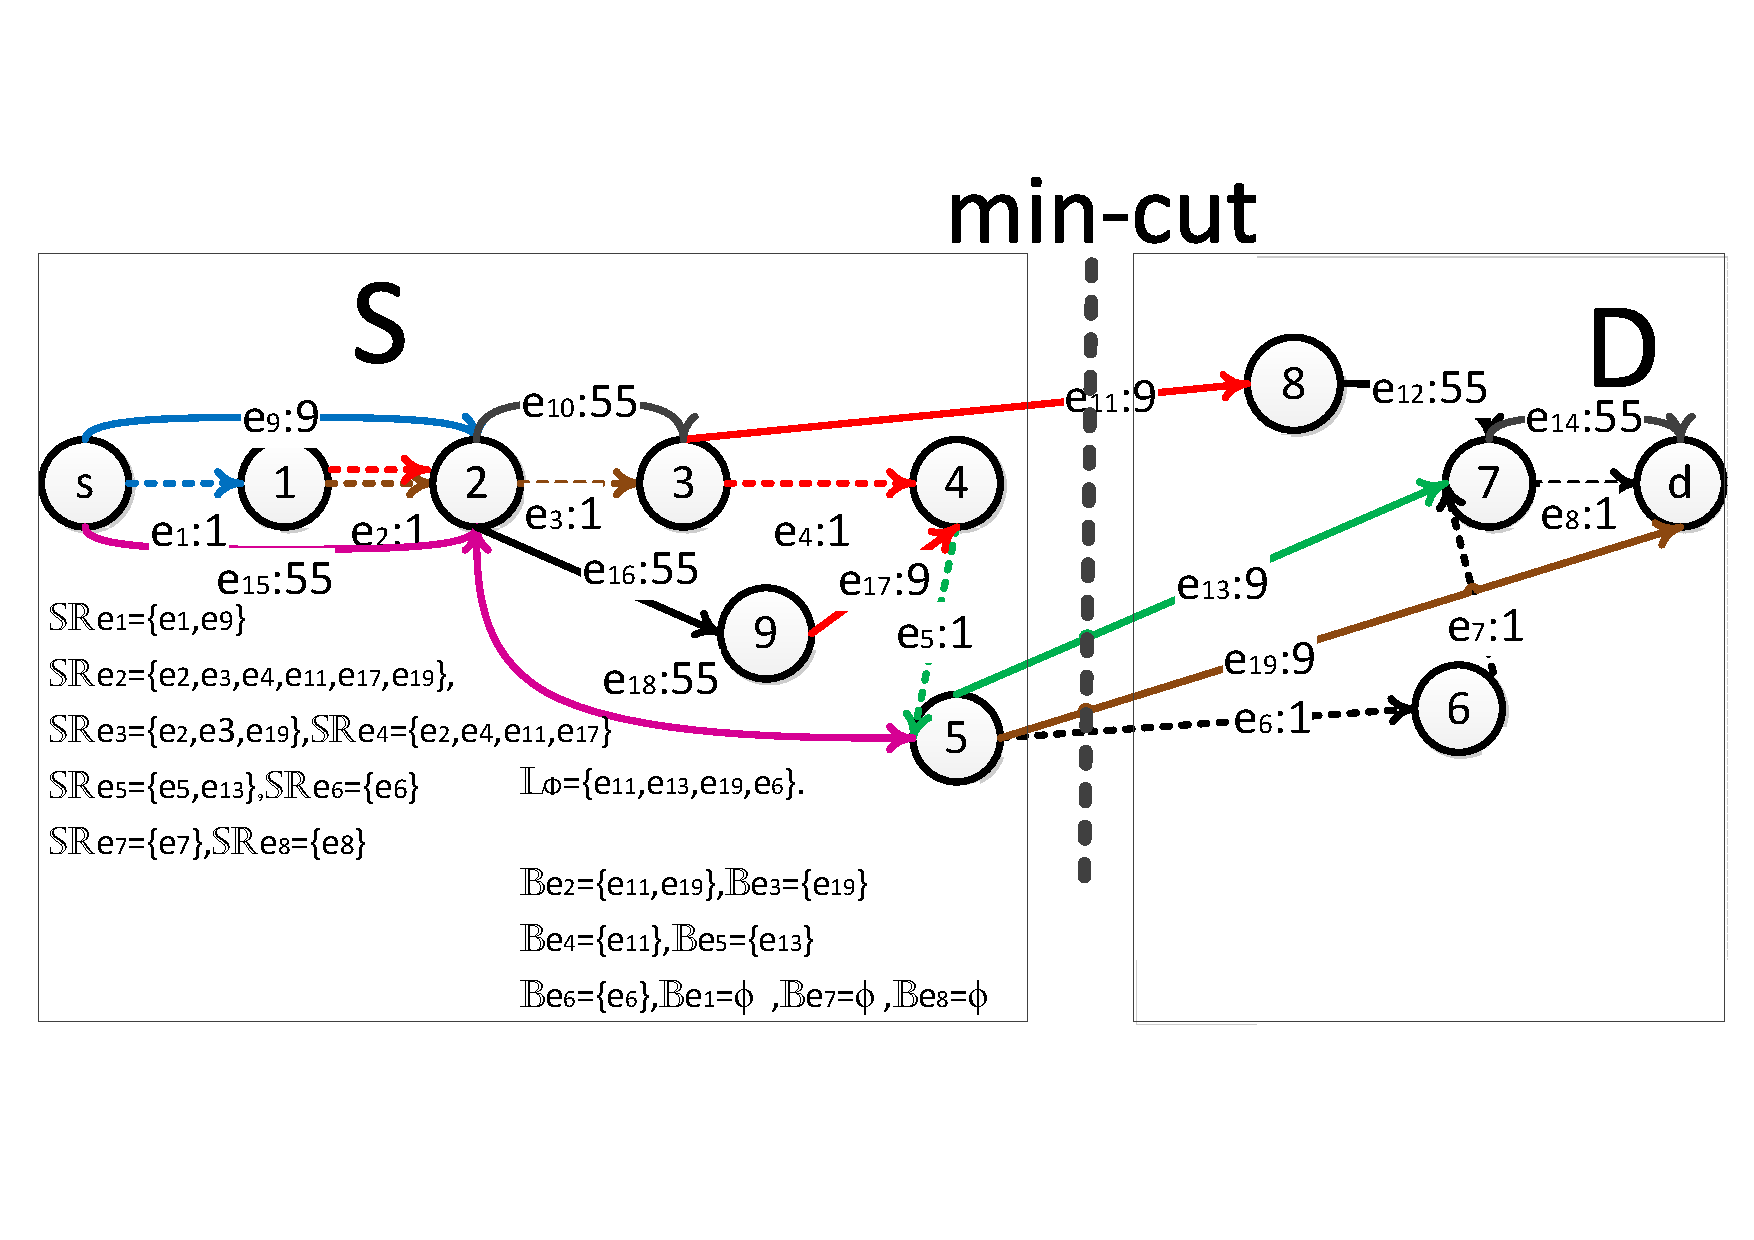
\includegraphics[width=1.35in]{franz/MinCutStarGraph}
  \caption{Min cut of Graph $G^*$, $\mathbb{SR}_{e_1}=\{e_1, e_9\},\mathbb{SR}_{e_2}=\{e_2,e_3,e_4, e_{11},e_{17},e_{19}\},\mathbb{SR}_{e_3}=\{e_2,e_3, e_{19}\},\mathbb{SR}_{e_4}=\{e_2,e_4, e_{11},e_{17}\},\mathbb{SR}_{e_5}=\{e_5, e_{13}\},\mathbb{SR}_{e_6}=\{e_6\},\mathbb{SR}_{e_7}=\{e_7\} $ and $\mathbb{SR}_{e_8}=\{e_8\}$. $\mathbb{L}_{\Phi}=\{e_{11},e_{13},e_{19},e_{6}\}$. $\mathbb{B}_{e_1}=\emptyset,\mathbb{B}_{e_2}=\{e_{11},e_{19}\},\mathbb{B}_{e_3}=\{e_{19}\},\mathbb{B}_{e_4}=\{e_{11}\},\mathbb{B}_{e_5}=\{e_{13}\},\mathbb{B}_{e_6}=\{e_6\}$,$\mathbb{B}_{e_7}=\emptyset$ and $\mathbb{B}_{e_8}=\emptyset$. \note{Dear sister, SR is wrong in this example, I will let the student to modify tomorrow}}\label{fig:MinCutStarGraph}
  \label{fig:MinCutStarGraph}
\end{figure*}

\begin{figure*}[tp]
\centering
% Requires \usepackage{graphicx}
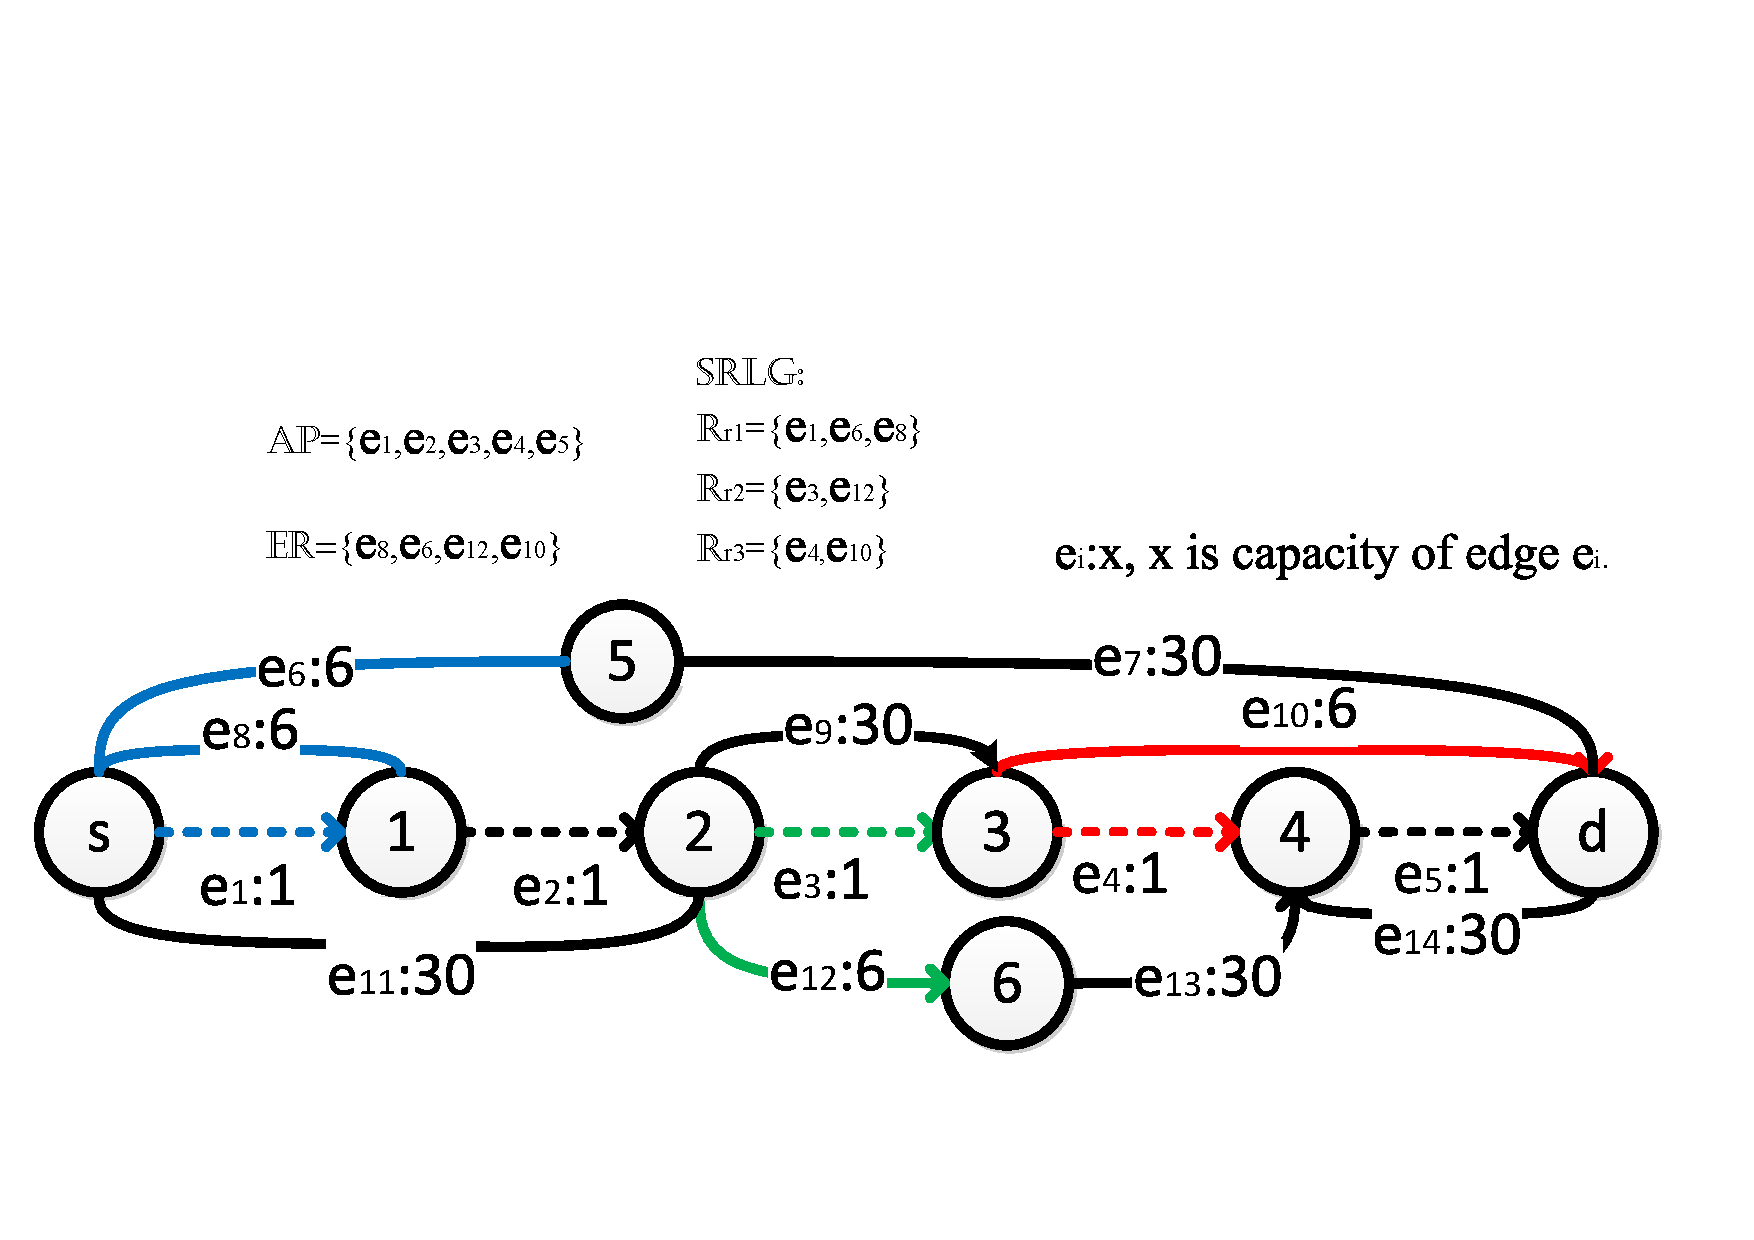
\includegraphics[width=1.35in]{franz/SampleTwoInitGraphFlowGraph}
\caption{Sample Graph $G^*_2$}\label{fig:SampleTwoInitGraphFlowGraph}
\end{figure*}
\begin{figure*}[tp]
\centering
% Requires \usepackage{graphicx}
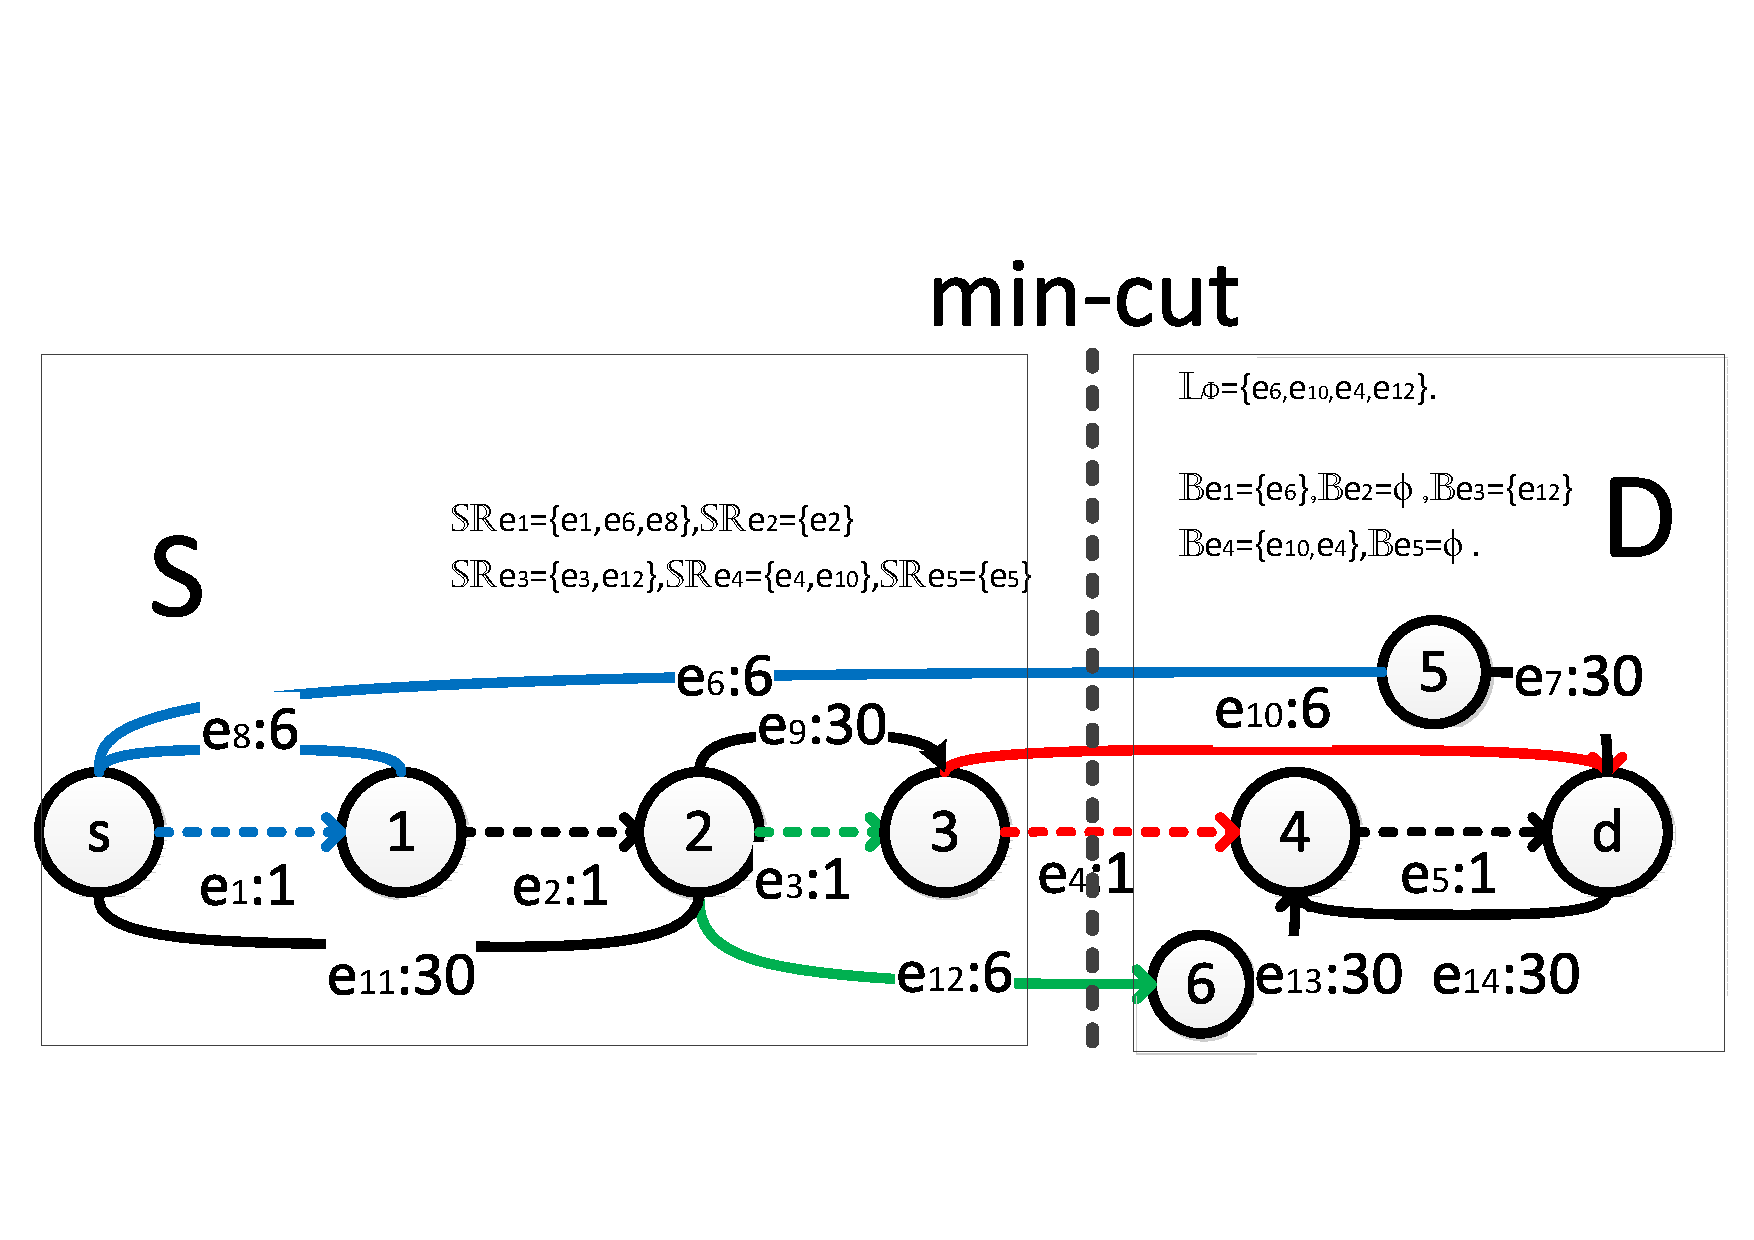
\includegraphics[width=1.35in]{franz/SampleTwoInitGraphCutGraph}
  \caption{Min cut of Sample Graph  $G^*_2$, $\mathbb{SR}_{e_1}=\{e_1,e_6,e_8\},\mathbb{SR}_{e_2}=\{\},\mathbb{SR}_{e_3}=\{e_3, e_{12}\},\mathbb{SR}_{e_4}=\{e_4, e_{10}\},\mathbb{SR}_{e_5}=\{e_5\}. \mathbb{L}_{\Phi}=\{e_{6},e_{10},e_{4},e_{12}\}. \mathbb{B}_{e_1}=\{e_6\},\mathbb{B}_{e_2}=\emptyset,\mathbb{B}_{e_3}=\{e_{12}\},\mathbb{B}_{e_4}=\{e_{10},e_4\}, \mathbb{B}_{e_5}=\emptyset$.}\label{fig:SampleTwoInitGraphCutGraph}
\end{figure*}
\begin{figure*}[tp]
\centering
% Requires \usepackage{graphicx}
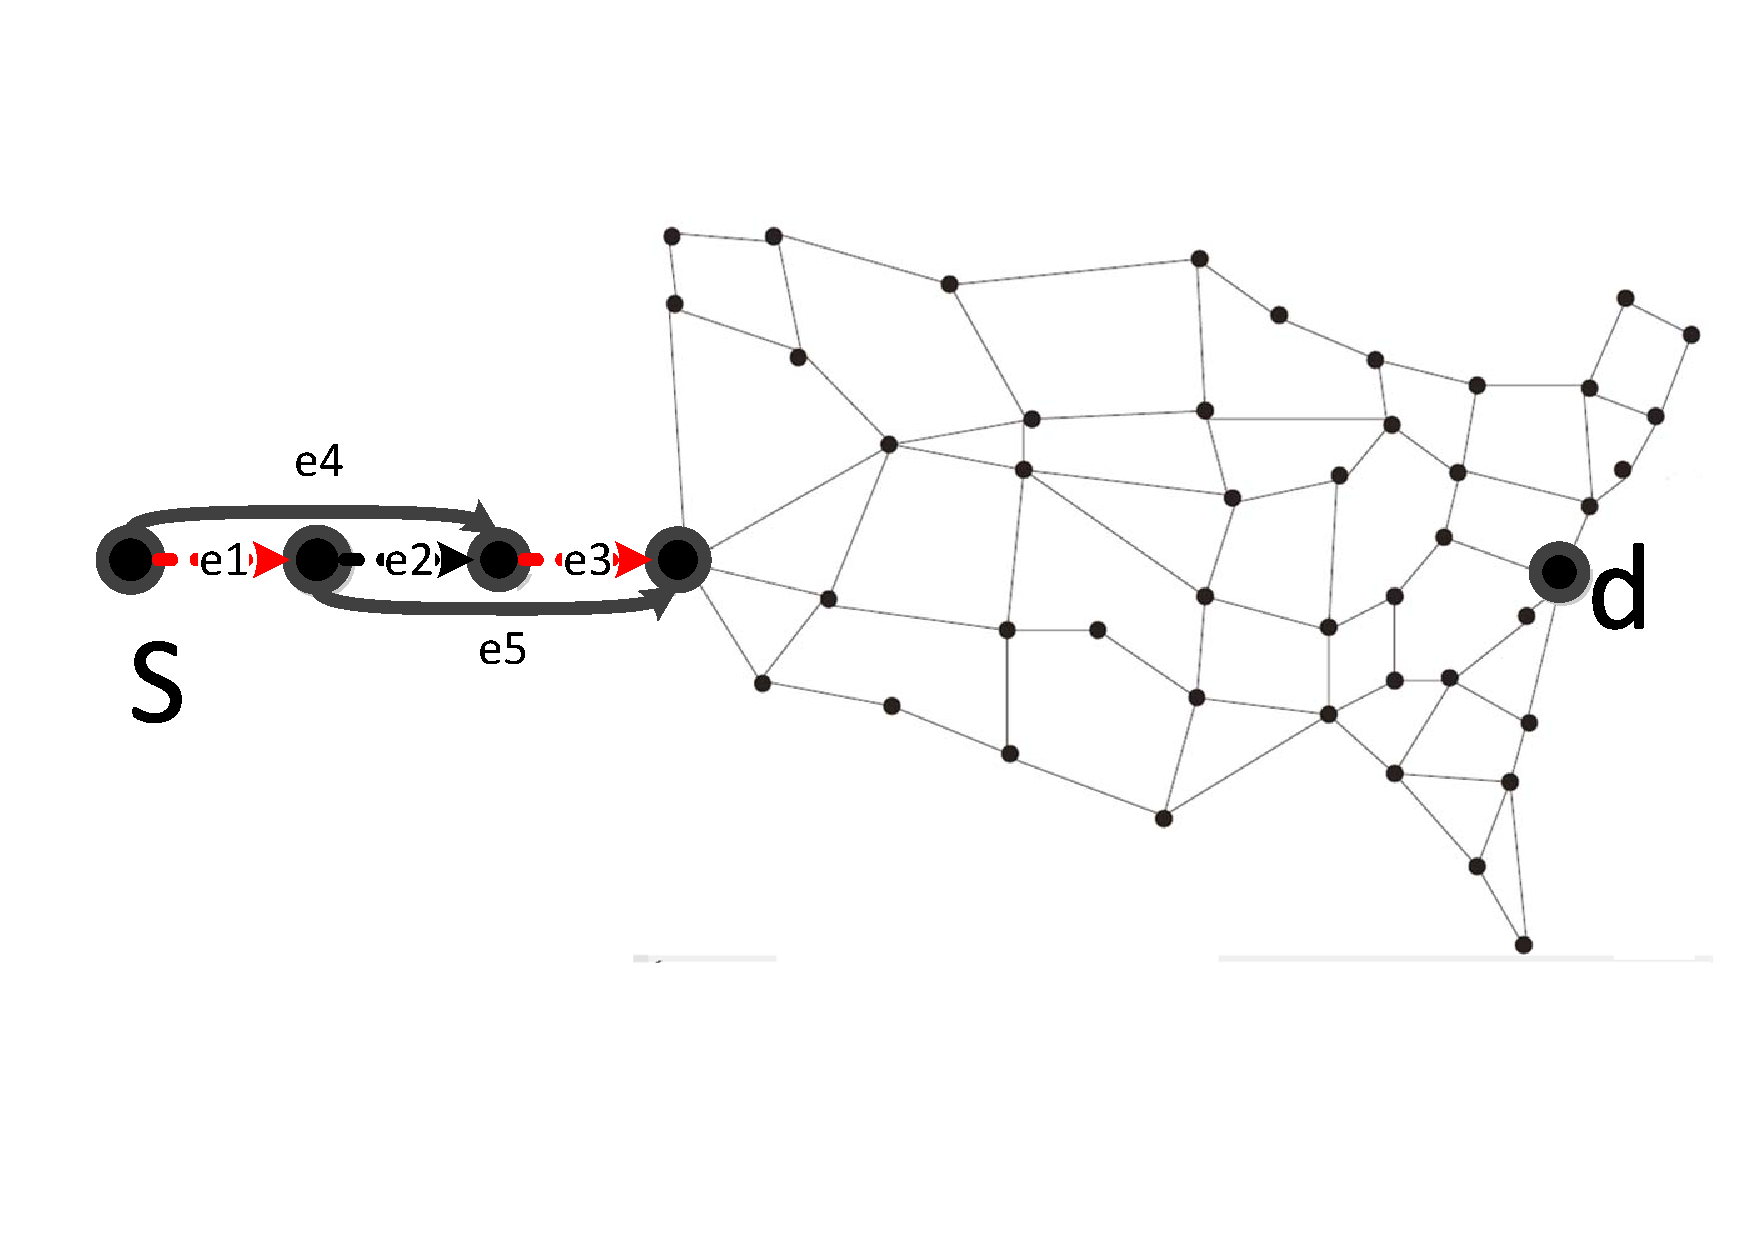
\includegraphics[width=1.35in]{franz/KSPproblem}
  \caption{In this graph, suppose SRLG conflicting set is ${e_1,e_3}$, When KSP algorithm find the $AP=(e_1,e_2,e_3,\ldots)$ iteratively, but the problemic edges $e_1,e_3$ always exist the k-th shortest path, then KSP could find the AP which is SRLG-disjoint with $BP$ in high time consumption. However, my algorithm find  problemic edges $e_1,e_3$ and find path AP in two subproblem $\mathcal{P}(\emptyset,\{e_1\})$ and $\mathcal{P}(\{e_1\},\{e_3\})$. $AP$ of the subproblem $\mathcal{P}(\emptyset,\{e_1\})$ pass edges $e_4$ and $e_3$ to destination $d$ with SRLG-disjoint path BP which pass edges $e_1$ and $e_3$ to destination $d$. In like manner, the subproblem $\mathcal{P}(\{e_1\},\{e_3\})$ could find disjoint paths pair. }\label{fig:KSPproblem}
\end{figure*}
\begin{figure}
  \centering
  % Requires \usepackage{graphicx}
  \includegraphics[width=2.35in]{franz/weight}\\
  \caption{Normalization Weitgh Value}\label{fig:normalization weitgh sum}
\end{figure}
\begin{figure}
  \centering
  % Requires \usepackage{graphicx}
  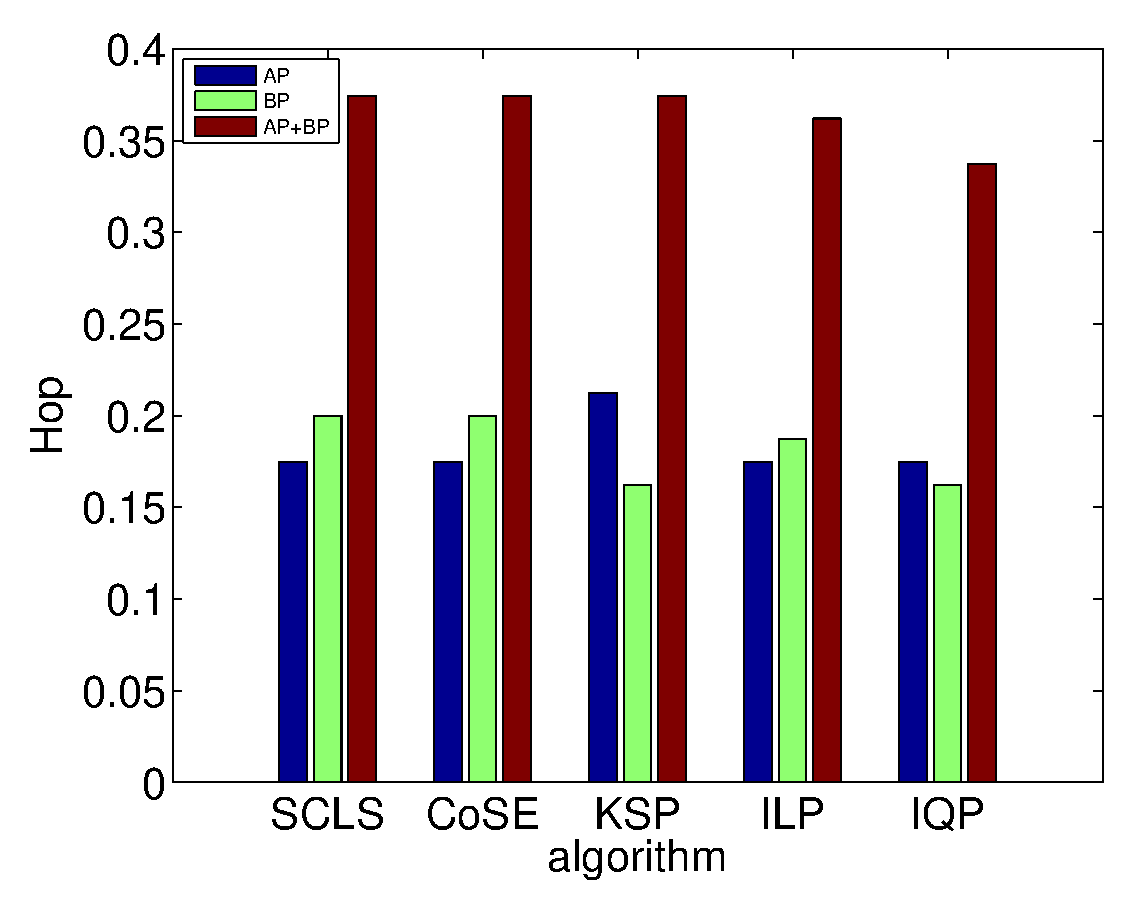
\includegraphics[width=2.35in]{franz/hop}\\
  \caption{Normalization Hop}\label{fig:normalization hop}
\end{figure}

\subsection{Runtime}
\begin{figure}
\centering
% Requires \usepackage{graphicx}
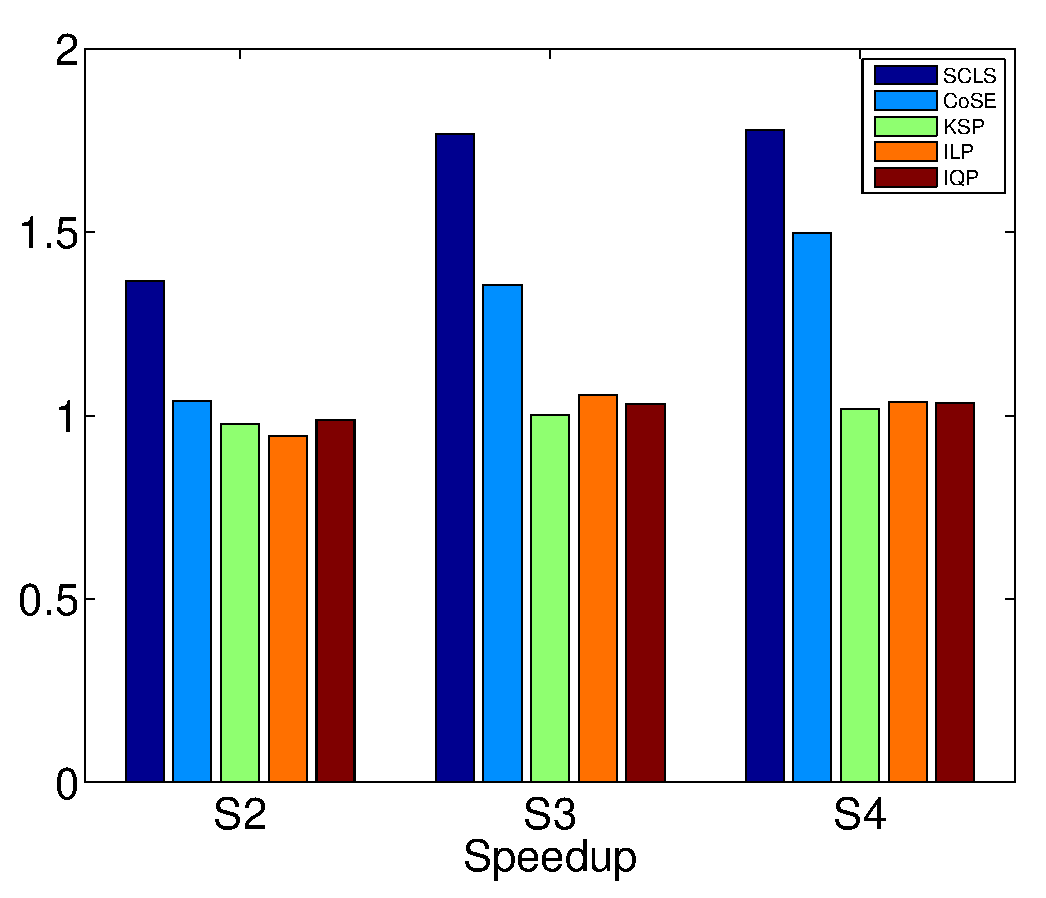
\includegraphics[width=1.35in]{franz/Speedup}\\
\caption{Speedup}\label{fig:Speedup}
\end{figure}
\begin{figure}
\centering
% Requires \usepackage{graphicx}
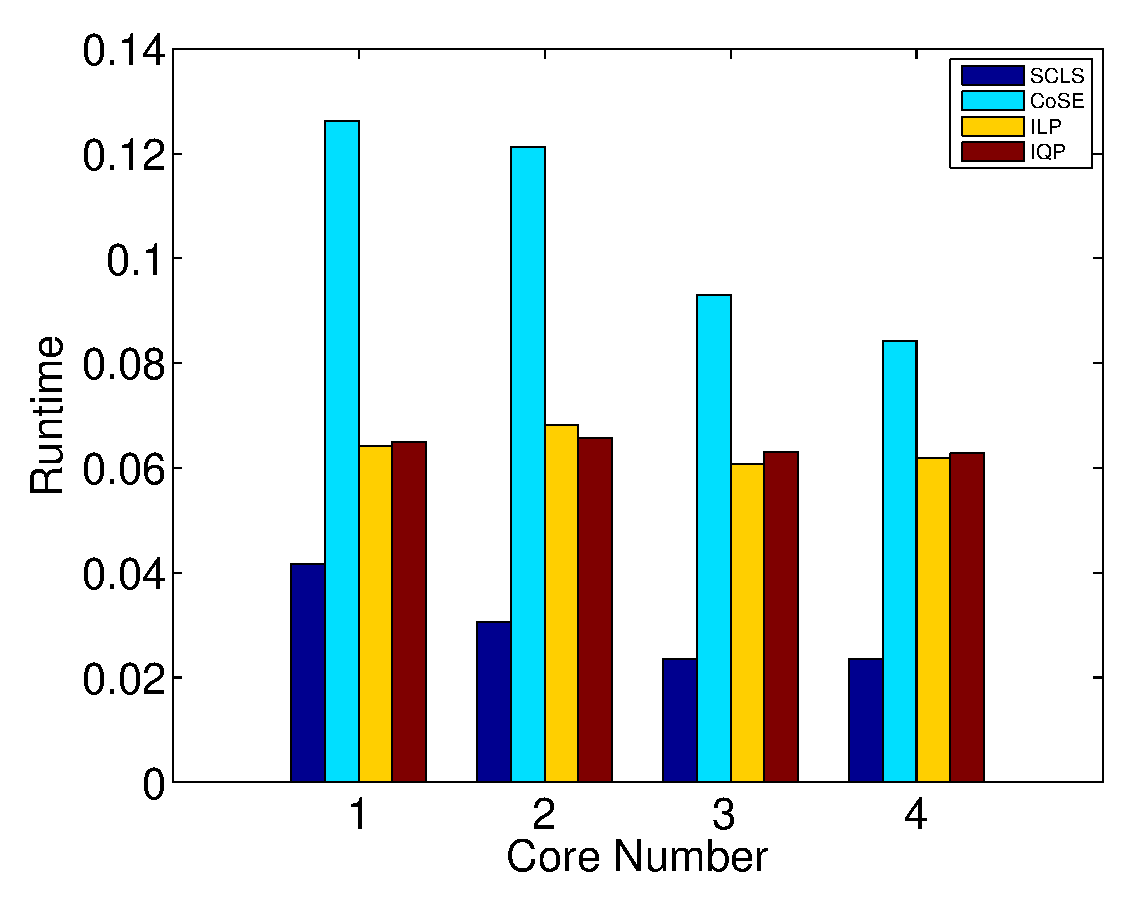
\includegraphics[width=1.35in]{franz/Runtime_NoKSP}\\
\caption{Runtime without KSP algorithm}\label{fig:Runtime_NoKSP}
\end{figure}
\begin{figure}
\centering
% Requires \usepackage{graphicx}
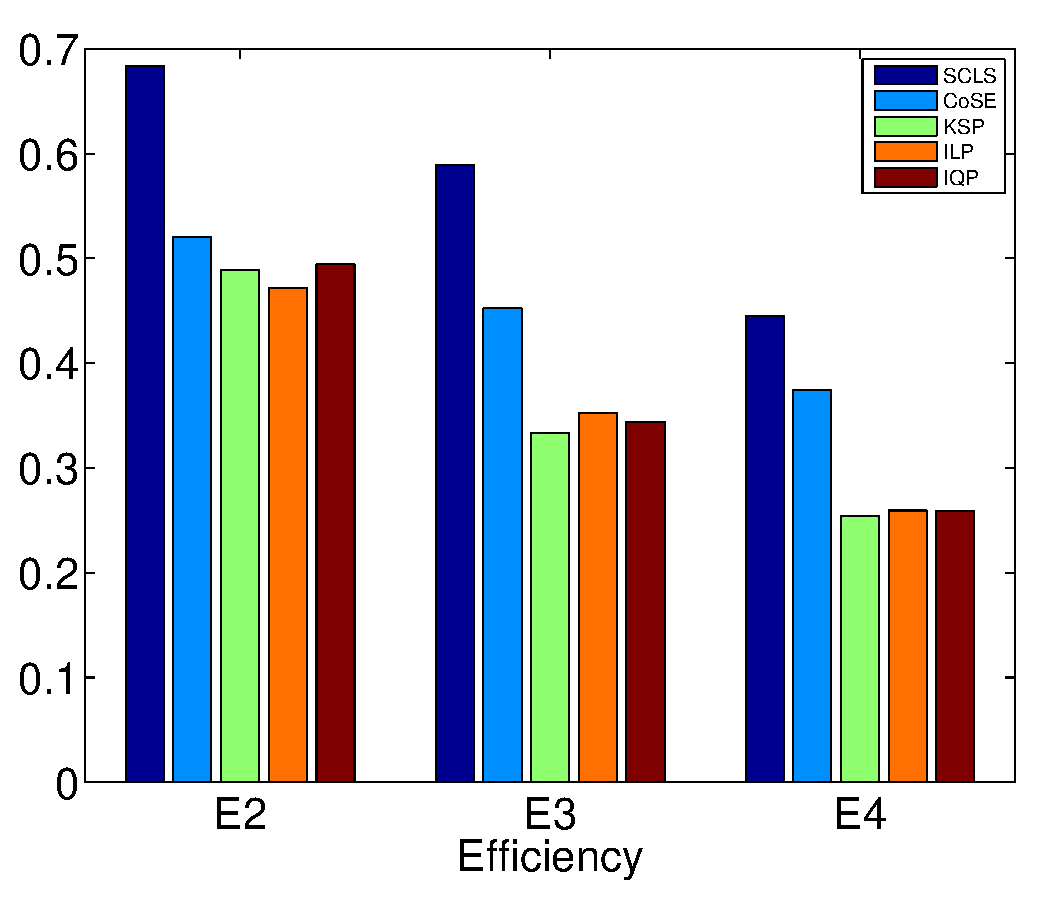
\includegraphics[width=1.35in]{franz/Efficiency}\\
\caption{Efficiency}\label{fig:Efficiency}
\end{figure}


\begin{table}
  \centering
  \begin{tabular}{*{7}{c}}
\toprule
Sample & 1 & 2 & 3 & 4 & 5 & 6 \\
\midrule
Node  & 424  & 1825 & 514&514 &8301 &1814   \\
Edge & 1378  & 24837 & 2024& 2074& 40326&24816  \\
\bottomrule
\toprule
Sample & 7&8&9&10&11&12 \\
\midrule
Node  &2014 & 2014&2014 & 2014& 2013&20 \\
Edge &2068 &2068 & 2068& 2068& 15661 & 31\\
\bottomrule
\toprule
Sample  &13&14&15&16&17 \\
\midrule
Node  &2014 &2014 & 424&2014 & 2014 & \\
Edge & 2068& 2068&1378 & 2068&2068& \\
\bottomrule
\end{tabular}
\caption{node number and edge number of all samples.}
\label{tab:AllSample}
\end{table}


\begin{algorithm}
\caption{Min-Min}
\begin{algorithmic}[1]
\label{alg:min-min}
%\caption{Main process of Algorithm}
\REQUIRE
$G$: the network graph\\
$s$: the source node\\
$d$: the destination node \\
$\mathbb{I}$:   the inclusion link set should be included in AP\\
$\mathbb{O}$: the exclusion link set should not be included in AP\\
\ENSURE
AP: the active path\\
BP: the backup path
\STATE $AP=\emptyset$, $BP=\emptyset$
\STATE $AP\leftarrow$ FIND$\_$AP$(G,s,d,\mathbb{I},\mathbb{O})$
\IF{$AP\neq\emptyset$}
    \STATE $BP\leftarrow$ FIND\_SRLG\_Disjoint\_BP$(G,s,t,AP)$
    \IF{$BP\neq\emptyset$}
        \STATE return path pair $(AP,BP)$
    \ELSE
        \STATE find SRLG conflict link set $\mathbb{T}$
        \STATE $\mathbb{T}\leftarrow \mathbb{T}-(\mathbb{I}\cup\mathbb{O})$
        %\IF{$\mathbb{T}\neq \emptyset$}
        \STATE {divide and conquer for execution in parallel\\
        \tiny{
        $\!\!\!\!\!\!\!\!\!\!\!\!\!\!\!\!\!\!\!\left\{ \begin{array}{l}
 \left( {A{P_1},B{P_1}} \right)={{Min-Min}}\left( {G,s,d,\mathbb{I} ,\mathbb{O}\cup\{ {t_1}\} } \right), \\
 \left( {A{P_2},B{P_2}} \right)={{Min-Min}}\left( {G,s,d,\mathbb{I}\cup\{ {t_1}\} ,\mathbb{O}\cup\{ {t_2}\} } \right), \\
 \left( {A{P_3},B{P_3}} \right)={{Min-Min}}\left( {G,s,d,\mathbb{I}\cup\{ {t_1},{t_2}\} ,\mathbb{O}\cup\{ {t_3}\} } \right), \\
  \cdots  \\
 \left( {A{P_{\left| \mathbb{T} \right|}},B{P_{\left| \mathbb{T} \right|}}} \right) = {{Min-Min}}\left( {G,s,d,\mathbb{I}\cup \{ {t_1},{t_2}, \cdots ,{t_{\left| \mathbb{T} \right| - 1}}\} ,\mathbb{O}\cup\{ {t_{\left| \mathbb{T} \right|}}\} } \right) \\
 \end{array} \right.$
 }
        }
        \STATE{  {$\!\!\!\!\!\!\!\!\!\!\!F\leftarrow$ FIND\_Feasible$(( {A{P_1},B{P_1}} )),\cdots,( {A{P_{|\mathbb{T} |}},B{P_{| \mathbb{T} |}}} )$}}
        %\ENDIF
         \IF{$F\neq{\emptyset,\emptyset}$}
         \STATE{return path pair $(AP,BP)$ satisfying that $AP = \mathop {\arg \min }\limits_{AP} \left\{ F \right\}$}
        \ENDIF

    \ENDIF
\ENDIF
\end{algorithmic}
\end{algorithm}
%\caption{算法步骤图}\label{fig:algorithm}

